\documentclass[10pt,twocolumn]{article}
\usepackage[letterpaper,margin=0.72in]{geometry}
\usepackage[T1]{fontenc}
\usepackage{lmodern,microtype,amsmath,amssymb,booktabs,graphicx,xcolor}
\usepackage[numbers,sort&compress]{natbib}
\usepackage[colorlinks=true,allcolors=blue]{hyperref}
\usepackage{enumitem,float}
\setlength{\columnsep}{0.25in}
\title{From Authorship Readout to Generation Control:\\A Controlled Residual-Stream Study of ``AI-Like'' Writing}
\author{Autonomous research study\\\small Reproducible code, raw generations, and ratings accompany this manuscript}
\date{}
\begin{document}
\raggedbottom
\maketitle
\begin{abstract}
Does a residual-stream direction that separates human and machine text control AI-like writing independently of register and answer quality? We fit paired, length-controlled directions in Qwen2.5-1.5B base and instruct models, then evaluate 1,140 answers under 19 interventions and 120 answers in a cross-corpus replication. The instruct mean direction achieves 0.992 held-out HC3 AUROC and about 0.89 on two HAP-E generators; base-model readout is similarly strong. Positive versus negative steering changes a historical detector by 0.248 [0.149, 0.355], with effects surviving nuisance orthogonalization. A supplemental contemporary detector corroborates score shifts, but almost all outputs remain detected. A late blinded Claude audit finds an AI-style contrast of 5.67 [2.90, 8.93] points, attenuated to 1.40 [0.00, 3.20] after nuisance removal, while formality steering has a larger point estimate. Strong negative steering reduces adequacy; style improvements are unresolved on the small quality-qualified subset. A cross-corpus direction also moves the two trained detectors in opposite directions. The evidence supports causal detection-related features, but does not establish a distinct, quality-preserving, human-perceived ``AI-ness'' axis.
\end{abstract}

\section{Introduction}
A model can distinguish human-written from machine-written text without possessing a single causal control for sounding machine-written. A readout may combine formatting, discourse conventions, register, subject matter, or fluency. Moreover, representations used while reading an isolated passage need not have the same function while generating an answer in a conversation. Establishing linear separability therefore leaves a mechanistic question unresolved: does intervening along a separating direction change perceived authorship while preserving useful content?

We study this question in Qwen2.5-1.5B, comparing base and instruction-tuned representations and intervening in the instruction-tuned model. We use question-matched, length-controlled human/ChatGPT excerpts to estimate a dense mean-difference direction. We test transfer to human and machine continuations of identical prefixes from two other generators. For generation, we vary intervention sign and magnitude, compare equal-norm random and nuisance directions, remove a nuisance subspace, ablate the centered authorship projection, and include a simple human-style prompt.

Our estimand is the paired change in external scores caused by a specified activation intervention on a fixed set of questions. It is not the probability that a text was actually written by a human: all generated answers have machine provenance. We distinguish causal changes in a detector's output from identification of a unique ``AI-ness'' representation. The latter requires specificity, external agreement, and preserved quality, beyond the fact that an intervention changes wording.

\section{Related work}
\paragraph{Authorship readout.} Quaremba et al.~\cite{quaremba2026} study linear probes for machine-text detection and a shared latent machine-text direction. SV-Detect~\cite{vishnyakov2026} uses per-layer human--machine directions and their alignment features to construct a detector. These results motivate the readout construction here, but detection performance alone does not validate an intervention during decoding.

\paragraph{Prior generative interventions.} Kuznetsov et al.~\cite{kuznetsov2025} analyze Gemma residual-stream SAE features for detection and explicitly steer selected decoder features during generation. Their feature interpretations include sophistication, expansion, and domain-specific behavior; their analysis also emphasizes length and formatting artifacts. Thus generative manipulation of detection-related features is already established. Our narrower experiment evaluates a dense paired authorship vector with independently scored outcomes and matched control interventions. We do not claim the first causal study of detection features.

\paragraph{Steering and persona.} Activation addition~\cite{turner2023} and contrastive activation addition~\cite{rimsky2023} motivate our inference-time vector interventions. Lu et al.~\cite{lu2026} identify an Assistant Axis using a broad collection of personas and show that persona interventions change behavior. Our small assistant-versus-storyteller contrast is a nuisance \emph{proxy}, not a replication of that axis. Disentangling it cannot establish independence from the full persona space.

\paragraph{Corpora and detection.} HC3~\cite{guo2023} supplies human and ChatGPT answers to common questions; its different writing communities remain a potential confound. HAP-E~\cite{reinhart2024} supplies human continuations and model continuations of the same preceding text, with a prompt requesting stylistic continuity. We also evaluate a frozen RoBERTa detector released for GPT-2 outputs~\cite{solaiman2019}. Its historical training distribution makes empirical validation necessary; it is not an authorship oracle.

\section{Method}
\subsection{Paired data and representations}
We select the first answer from each author class meeting a minimum of 96 Qwen tokens. Before tokenization, we collapse whitespace, remove whitespace before punctuation, and join selected spaced English contractions. We use the first 96 tokens of each answer, with no question, chat template, or authorship label in the representation-extraction input. All retained excerpts retokenize to exactly 96 tokens. We deduplicate normalized questions and exact excerpts before splitting.

Our HC3 subset contains 500 training, 100 validation, and 200 test question pairs, balanced across finance, medicine, Reddit ELI5, and computer science/AI. Each pair contributes one human and one ChatGPT excerpt. Open-domain QA is excluded because only 41 pairs meet the length threshold, insufficient for the balanced design. Splits are disjoint by question, and train/validation/test have no exact excerpt overlap. The pre-outcome protocol and data-integrity amendments are included in the artifacts.

For transfer, we sample 180 shared HAP-E documents, 30 from each of its six registers. We compare the human \emph{second} chunk, not the prompting first chunk, with GPT-4o-mini and Llama-3-8B-Instruct continuations. Each generator comparison has 180 human and 180 machine excerpts; the human excerpts are shared across comparisons. All transfer excerpts receive the same normalization and 96-token cap. Transfer documents are never used to fit or select a direction.

We use public Qwen2.5-1.5B base and instruct checkpoints~\cite{qwen2024}, with bfloat16 inference. Let $h_{\ell,t}(x)$ denote the residual after transformer block $\ell$ for token $t$ of excerpt $x$. We compute
\begin{equation}
 z_\ell(x)=\frac{1}{96}\sum_{t=1}^{96}h_{\ell,t}(x),\quad
 d_\ell=\frac{1}{N}\sum_{i=1}^N[z_\ell(a_i)-z_\ell(b_i)],
\end{equation}
where $a_i$ is the machine answer and $b_i$ its human counterpart. We evaluate scalar scores $z_\ell(x)^\top d_\ell$ and an L2 logistic probe ($C=1$, unstandardized features, intercept) at blocks 7, 14, and 21. The intervention block maximizes validation AUROC of the \emph{instruct mean direction}, with the earlier block winning ties. Logistic probes do not define our intervention. Base/instruct comparisons use the same data and blocks; we do not transfer an instruct vector into base coordinates.

\subsection{Interventions and controls}
For greedy decoding, we intervene after a single block:
\begin{equation}
 h'_{\ell,t}=h_{\ell,t}+\alpha d_\ell.
\end{equation}
The hook acts on all prompt positions during prefill and on each new token during cached decoding. We test $\alpha\in\{-2,-1,-0.5,0,0.5,1,2\}$. These units are multiples of the empirical class-mean difference, not residual standard deviations. Two Gaussian control directions (seeds 101 and 202) are each normalized to $\|d_\ell\|_2$ and tested at signs $\pm1$.

To estimate nuisance directions, we generate answers to 40 \emph{training} questions, ten per domain, under four prompts: formal academic register, casual conversational register, helpful professional AI assistant, and whimsical fictional storyteller. Each requests an accurate answer of about 80 words. We re-encode normalized answer text alone, mean-pooling up to its first 96 tokens. Formal-minus-casual and assistant-minus-storyteller means define register and persona-proxy directions. Both are rescaled to $\|d_\ell\|_2$ and tested at $\pm1$. These interventions control for the effect of their specified contrasts, not all possible forms of formality or identity.

We also form train-only covariance directions for log original answer length and instruct-model negative log likelihood (NLL), subtracting the within-authorship-class means of both the covariate and activations first. This avoids defining these nuisance vectors solely by class membership. Three domain-centroid contrasts complete the nuisance span. With $Q$ an orthonormal basis for these seven vectors, we define
\begin{equation}
 d_{\perp}=\|d\|_2\frac{(I-QQ^\top)d}{\|(I-QQ^\top)d\|_2},
\end{equation}
and test it at $\pm1$. Equal norm makes this a directional specificity test, not a comparison of smaller perturbations. Orthogonality is a geometric constraint and does not guarantee semantic independence after nonlinear downstream computation.

For centered projection ablation, $u=d/\|d\|_2$ and $c$ is the midpoint of training class means:
\begin{equation}
 h'=h-u[u^\top(h-c)].
\end{equation}
This sets each intervened token's projection to the midpoint. It is distinct from subtracting a constant vector. Finally, a no-hook prompt baseline adds: ``Write like a human, with natural wording rather than a typical AI-generated answer.''

\subsection{Generation and external evaluation}
We use 60 held-out HC3 questions, 15 per domain, with the same question in every condition. The standard instruction asks for a clear answer in one short paragraph of about 80 words. Greedy decoding permits at most 160 new tokens. There are 19 conditions and 1,140 generated answers, plus 160 nuisance-control answers. Conditions are not selected using detector outcomes.

We score complete generated answers with the frozen \texttt{roberta-base-openai-detector}, taking the softmax score for its \texttt{Fake} label (maximum 512 detector tokens). Independently, Mistral-7B-Instruct-v0.3~\cite{jiang2023} receives the question and anonymous answer, without intervention identifiers or provenance labels. It assigns AI-like \emph{style} on a 0--100 scale, coherence, answer adequacy, and formality on 1--5 scales. Adequacy explicitly asks about correctness and relevance. The judge is instructed to ignore excerpt truncation alone but penalize repetition, nonsensical language, and factual errors. Full prompts and raw completions are preserved. Neither evaluator uses the Qwen activations or trains on the fit split.

The local judge replaced the planned API judge because the provided OpenRouter endpoint rejected requests due to a daily key limit and the fallback OpenAI key was invalid. The initial study used no successful API ratings. After the UTC-day quota reset, a late Claude Haiku 4.5 audit evaluated the already fixed outputs with the same rubric; Section~\ref{sec:claude} reports it separately. A local judge is an imperfect automated measure; in particular, correctness scores are not expert fact checks. We audit both evaluators on 80 held-out HC3 pairs and 30 HAP-E document triplets (250 texts total). This audit involves no fitting or threshold tuning.

\subsection{Analysis and quality controls}
We report mean outcomes and within-question changes relative to baseline, with percentile bootstrap confidence intervals from 2,000 question-level resamples. For readout AUROC, bootstrap units are question pairs or HAP-E documents. Confidence intervals are exploratory and uncorrected for multiple comparisons. We also compare positive and negative interventions directly, holding questions fixed.

Primary quality comparisons use Mistral ratings; the late audit repeats them using Claude. A quality-qualified pair requires coherence $\geq4$ and adequacy $\geq4$ for both the baseline and modified answer. We report its size and score changes, alongside the unconditional analysis. This is a descriptive quality filter, \emph{not} a causal adjustment: conditioning on post-intervention quality can select different questions in different conditions. It cannot establish equivalence or content preservation on the original prompt population.

We record generated length, repeated word-trigram fraction, and unmodified base-Qwen NLL on the first 96 tokens. A supplemental frozen-detector analysis uses exactly 64 Qwen tokens when both outputs are long enough. This checks a length explanation but again conditions on post-treatment eligibility. Leave-one-domain-out readout refits the mean direction on three training domains and evaluates the fourth test domain. Software checks verify split integrity, equal control-vector norms, nuisance orthogonality, and agreement between hidden-state indexing and the intervention hook.

\section{Results}
\subsection{Readout transfers without consistent chat amplification}
Validation selects block 21 (mean-direction AUROC 0.989). At that block, the instruct mean direction achieves HC3 test AUROC 0.992, with 0.893 and 0.885 on HAP-E GPT-4o-mini and Llama-3-8B-Instruct, respectively. The corresponding base-model results are 0.993, 0.896, and 0.869. Logistic probes further improve separability (Table~\ref{tab:readout}). These measurements support a transferable readout, but not a consistent amplification from instruction tuning. Base/instruct differences vary by generator and readout. No base-model generation intervention is tested.

\begin{table*}[t]
\centering\small
\resizebox{\textwidth}{!}{\begin{tabular}{llccc}
\toprule
Model & Readout & HC3 & HAP-E GPT-4o-mini & HAP-E Llama-3-8B-I \\
\midrule
Base & Mean difference & 0.993 [0.985, 0.999] & 0.896 [0.872, 0.921] & 0.869 [0.843, 0.897] \\
Base & Logistic & 0.999 [0.998, 1.000] & 0.896 [0.868, 0.922] & 0.915 [0.888, 0.939] \\
Instruct & Mean difference & 0.992 [0.984, 0.998] & 0.893 [0.870, 0.918] & 0.885 [0.859, 0.911] \\
Instruct & Logistic & 0.999 [0.998, 1.000] & 0.898 [0.871, 0.924] & 0.936 [0.913, 0.957] \\
\bottomrule
\end{tabular}
}
\caption{Readout AUROC at the validation-selected block 21, with paired/document bootstrap 95\% intervals. HC3 has 200 test pairs; each HAP-E comparison has 180 document pairs. Logistic probes and mean-difference vectors are fit on the same 500 HC3 training pairs.}
\label{tab:readout}
\end{table*}
\begin{figure}[t]
\centering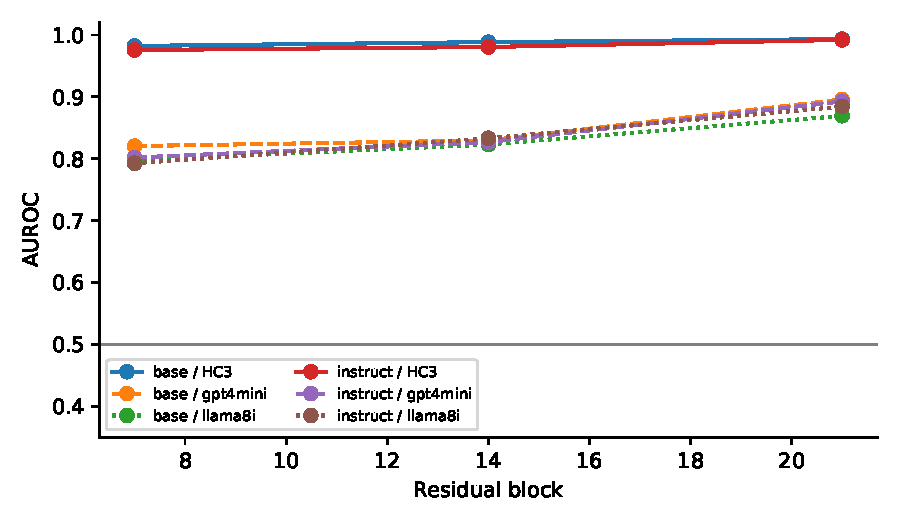
\includegraphics[width=\columnwidth]{figures/readout.pdf}
\caption{Mean-direction readout by block. Transfer remains above chance for both base and instruct models; chat tuning does not uniformly improve it.}
\label{fig:readout}
\end{figure}

Leave-one-domain-out mean-direction AUROCs range from 0.978 to 0.999 for instruct and from 0.983 to 1.000 for base (appendix). Thus the HC3 readout is not merely a classifier of the four domain labels. Matching and normalization cannot eliminate every within-domain discourse or collection artifact, however.

\subsection{A causal detector effect, with asymmetric quality costs}
In the primary sweep, quality ratings and filters use Mistral; the late audit below supplies a stricter independent assessment. Positive HC3 authorship steering raises the legacy RoBERTa score from 0.368 at baseline to 0.554 at $+1$ and 0.700 at $+2$. Paired changes are $+0.186$ [0.082, 0.292] and $+0.332$ [0.220, 0.448]. The $+1$ minus $-1$ contrast is $0.248$ [0.149, 0.355]. Because questions, decoding, and prompts are fixed, this identifies an effect of the specified residual intervention on the downstream score.

The reverse intervention is less persuasive as a humanization method. At $-1$, the score falls by 0.062, with an interval crossing zero [$-0.168$, 0.045]. At $-2$, it rises slightly rather than falling further. Adequacy drops by 0.600 points [$-0.900$, $-0.333$] and coherence by 0.333 [$-0.533$, $-0.150$]. Only 53 of 60 answers satisfy the automated quality threshold, compared with all 60 baseline answers. In contrast, positive $+1$ steering changes adequacy by 0.017 [$-0.100$, 0.117], with all answers passing. These are quality-proxy outcomes, not proof of factual equivalence.

\begin{figure*}[t]
\centering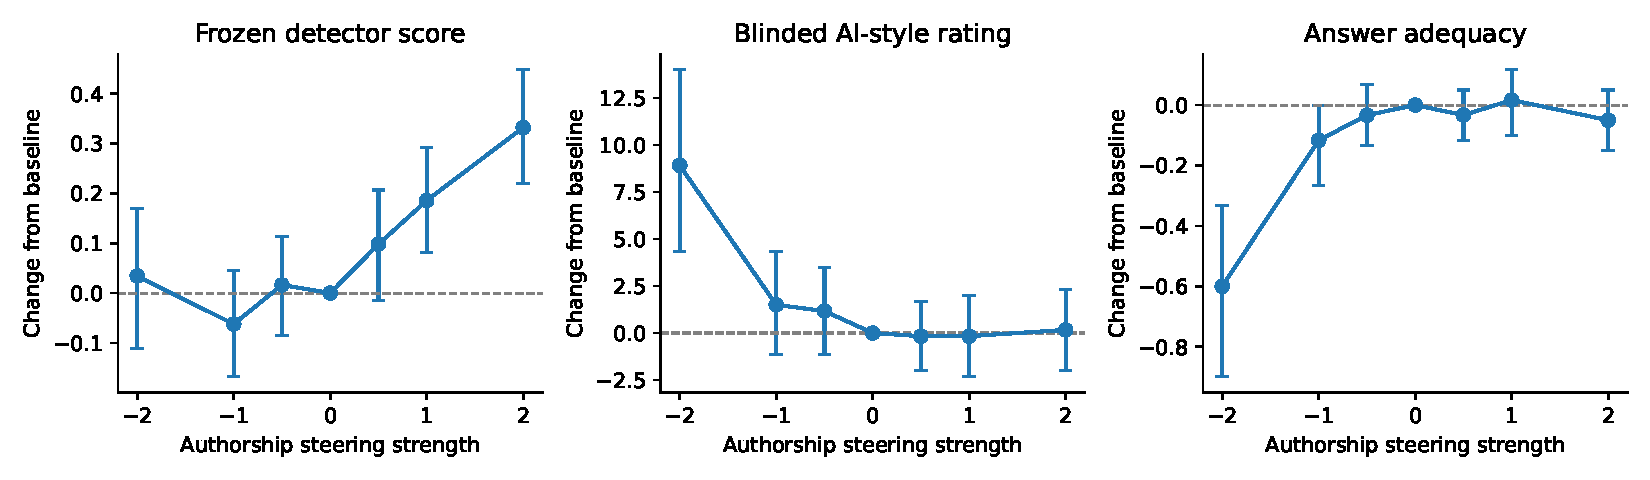
\includegraphics[width=\textwidth]{figures/dose.pdf}
\caption{Primary HC3-direction dose response, relative to the same-question baseline. Error bars are paired 95\% bootstrap intervals. The AI-style judge is unsuccessful at provenance discrimination (Table~\ref{tab:calibration}), so its near-flat response cannot validate or refute perceptual humanization. Negative extreme steering reduces rated adequacy.}
\label{fig:dose}
\end{figure*}

Centered ablation lowers RoBERTa by 0.132 [$-0.231$, $-0.031$], with mean adequacy change $-0.067$ [$-0.150$, 0.017]. The human-style prompt changes its score by $-0.062$ [$-0.162$, 0.035]. Both results are included alongside the full sweep, rather than choosing the best-performing intervention after observing outcomes. On exactly 64-token output prefixes, $+2$ retains a positive legacy-detector effect of 0.282 [0.166, 0.394], whereas the $+1$ interval crosses zero. Different eligibility sets and shorter evidence windows limit direct comparison with full answers.

\subsection{Specificity survives some, but not all, controls}
The authorship direction has cosine similarities 0.294 with formality, 0.261 with the persona proxy, 0.274 with original length, and $-0.292$ with the likelihood nuisance. Joint removal retains 89.0\% of its norm before rescaling. The orthogonalized direction still has a RoBERTa sign contrast of 0.206 [0.074, 0.334], with all 60 positive/negative pairs satisfying the quality criterion. This argues against those \emph{estimated linear nuisance axes} completely explaining the intervention.

Specificity is incomplete. The authorship sign effect exceeds the formality control by 0.362 [0.216, 0.504] and the persona proxy by 0.201 [0.033, 0.377]. It also exceeds random seed 101, but not conclusively random seed 202: the latter itself has a sign effect of 0.138 [0.027, 0.253], and the authorship-minus-random difference is 0.110 [$-0.042$, 0.272]. Two random directions are a limited sample of perturbation space. Figure~\ref{fig:controls} shows the control contrasts, and the appendix reports every condition.

\begin{figure*}[t]
\centering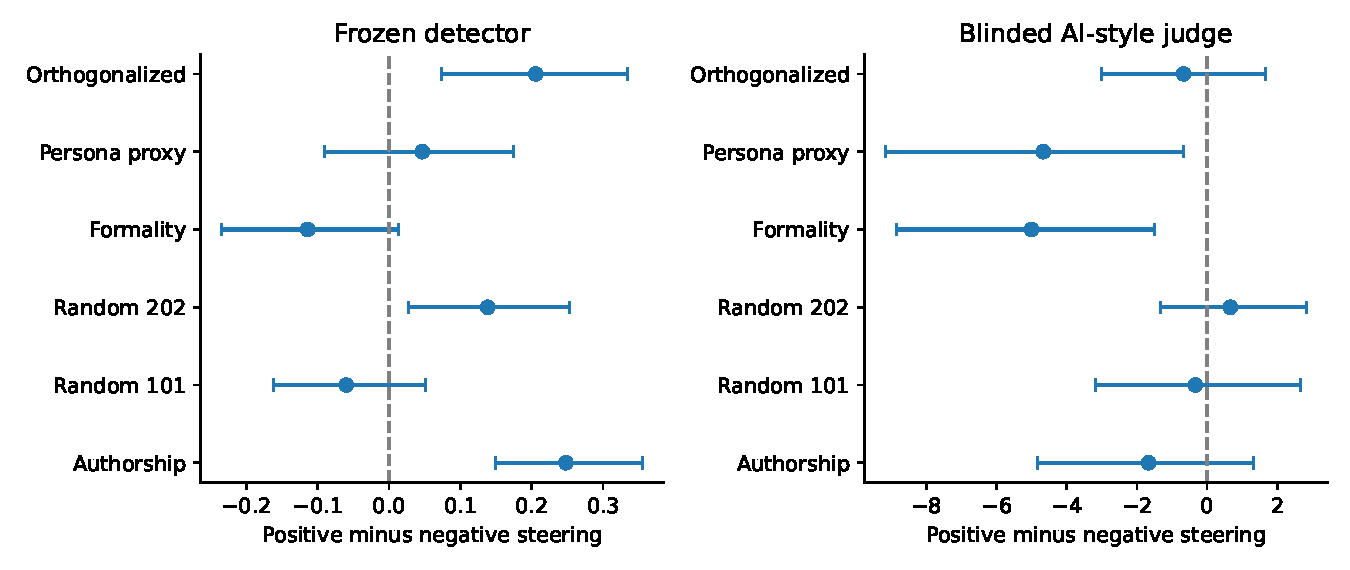
\includegraphics[width=0.93\textwidth]{figures/controls.pdf}
\caption{Positive minus negative equal-norm interventions at magnitude 1. The legacy detector responds to the authorship and nuisance-orthogonalized directions, but also to one random direction. The blinded style judge is not a reliable authorship detector on the audit sets.}
\label{fig:controls}
\end{figure*}

\subsection{Evaluator validity changes the interpretation}
The blinded judge fails our authorship-discrimination audit: its AI-style rating has AUROC 0.343 on HC3 and 0.434 on HAP-E, while assigning higher mean AI-style scores to human excerpts. We retain these ratings without reversing their sign, but do not use them as independent corroboration of an authorship effect. This audit does not supply ground-truth \emph{perceived} style labels; it shows that the chosen operational measure does not track known provenance in our samples.

We therefore added a separately labeled exploratory measure: the public Desklib DeBERTa-v3-large detector~\cite{desklib}. Its documented masked-mean-pooling sigmoid head was loaded with a strict weight-key check, without fitting or threshold tuning. On the same audit texts it achieves AUROC 0.992 on HC3 and 0.987 on HAP-E, compared with 0.933 and 0.658 for the historical RoBERTa detector (Table~\ref{tab:calibration}). Detector independence here means separate weights, architecture, and inference from the intervention model; unknown overlap in pretraining or detector training cannot be ruled out.

\begin{table}[t]
\centering\scriptsize\begin{tabular}{llrc}
\toprule
Dataset & Measure & Texts & AUROC [95\% CI] \\
\midrule
HAPE & RoBERTa & 90 & 0.658 [0.544, 0.761] \\
HAPE & Mistral judge & 90 & 0.434 [0.319, 0.553] \\
HC3 & RoBERTa & 160 & 0.933 [0.890, 0.971] \\
HC3 & Mistral judge & 160 & 0.343 [0.280, 0.406] \\
HC3 & Desklib & 160 & 0.992 [0.984, 0.998] \\
HAPE & Desklib & 90 & 0.987 [0.962, 1.000] \\
HC3 & Claude (late) & 160 & 0.856 [0.804, 0.903] \\
HAPE & Claude (late) & 90 & 0.849 [0.788, 0.906] \\
\bottomrule
\end{tabular}

\caption{Independent-measure audit on held-out natural texts. HC3 has 80 human/machine pairs; HAP-E has 30 document triplets. Intervals resample pairs/documents. Desklib was an exploratory addition.}
\label{tab:calibration}
\end{table}

Desklib scores are near ceiling on baseline generations (mean 0.990). At $-1$, the mean decreases by 0.024 [$-0.049$, $-0.004$]; the $+1$ minus $-1$ contrast is 0.028 [0.006, 0.056]. The orthogonalized sign contrast is likewise positive, 0.024 [0.008, 0.047]. Nevertheless, 58 of 60 $-1$ answers and all 60 baseline answers remain above the detector's conventional 0.5 cutoff. At $-2$, 59 remain above it. Shifting a continuous detection score is not equivalent to successful evasion.

Because sigmoid saturation obscures score movement, we additionally retained pre-sigmoid logits as an explicitly post-inspection diagnostic. The HC3 direction's $+1$ minus $-1$ logit contrast is 2.060 [1.410, 2.731], compared with 1.073 for formality, 0.105 for the persona proxy, and 0.097 and $-0.078$ for the two random directions. Its contrast exceeds formality by 0.987 [0.090, 1.897], and both random controls by intervals excluding zero. The orthogonalized logit contrast remains 1.840 [1.222, 2.483]. These exploratory results support a detection-related component beyond the fitted nuisance span, but depend on one added detector and cannot establish a universal perception axis.

The $-1$ Desklib logit shift remains negative on the 59 quality-qualified pairs ($-1.244$), and on fixed 64-token prefixes ($-1.051$ [$-1.800$, $-0.247$]). These checks reduce, but do not remove, concerns about length and gross quality. Figure~\ref{fig:modern} makes the sigmoid ceiling visible.

\begin{figure*}[t]
\centering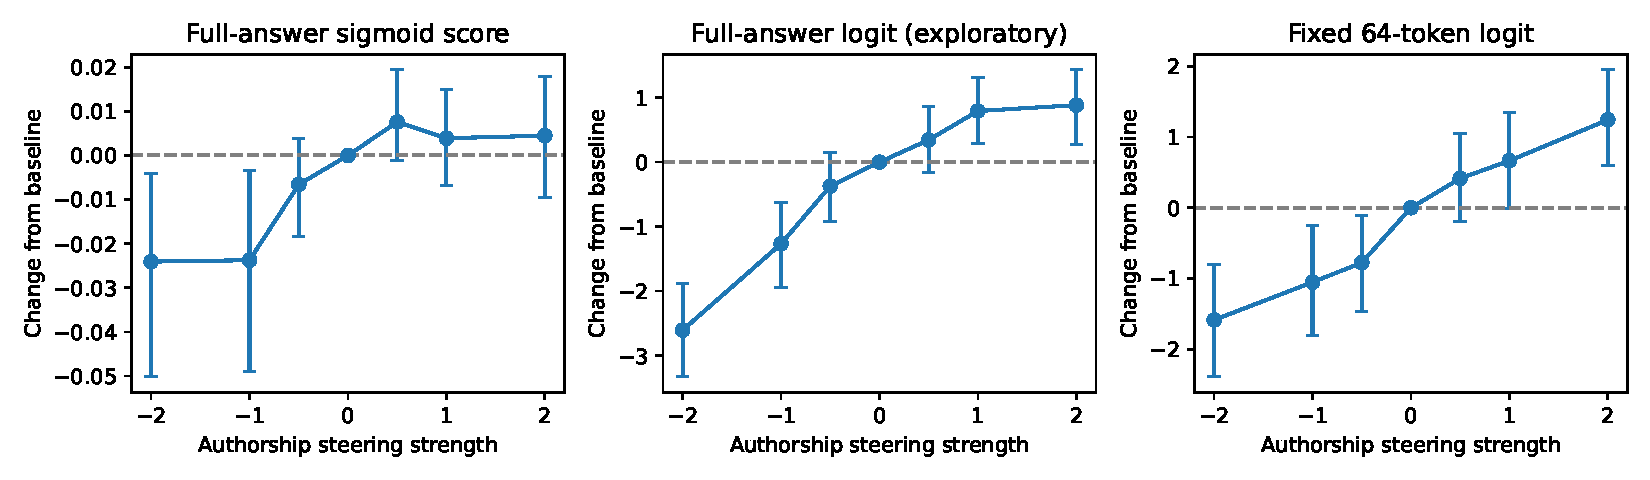
\includegraphics[width=\textwidth]{figures/modern_dose.pdf}
\caption{Exploratory Desklib outcomes. Sigmoid scores are near ceiling, so logit changes are more visible than probability-scale changes. Fixed-prefix eligibility is treatment-dependent. Logit analysis was added after inspecting saturation and is not a prespecified primary endpoint.}
\label{fig:modern}
\end{figure*}

We separately stress-tested the quality rubric on 20 baseline answers and 60 constructed corruptions, with unchanged blinded prompts. Mean coherence falls from 4.40 to 2.60 under word shuffling and to 1.60 under repetition; adequacy falls from 4.75 to 1.00 when an unrelated answer is substituted. Thus the rubric detects clear failures, even though its AI-style score does not track provenance. This audit validates sensitivity to gross corruption, not factual accuracy or subtle semantic preservation.


\subsection{Cross-corpus causal replication}
An exploratory replication fits a second mean direction on 180 additional HAP-E documents, disjoint from transfer-evaluation documents, with both machine generators contributing equally. We retain the HC3-selected block and match the HC3 vector norm. This vector has cosine 0.589 with the HC3 vector; its held-out AUROCs are 0.952 on HC3, 0.984 on HAP-E GPT-4o-mini, and 0.941 on HAP-E Llama. It therefore provides a plausible cross-corpus readout, not simply an arbitrary control.

Its 120 additional interventions reveal evaluator dependence. Positive HAP-E steering \emph{reduces} the historical RoBERTa score by 0.132 [$-0.231$, $-0.038$], whereas negative steering increases it by 0.137 [0.005, 0.271]. This reverses the expected sign despite positive geometric alignment. Desklib instead responds in the expected direction: the positive-minus-negative sigmoid contrast is 0.039 [0.009, 0.079], with logit contrast 2.712 [2.103, 3.321]. All 60 answers under either sign pass the coarse quality threshold. The same intervention can therefore increase one independently trained detector's notion of machine text and decrease another's.

Together, the HC3 and HAP-E experiments support a steerable, detection-related writing component. They do not identify an evaluator-invariant ``AI-ness'' variable. Table~\ref{tab:modernall} reports the exploratory detector results for every direction, including the transfer experiment, rather than only favorable comparisons.


\subsection{Late external style and quality audit}
\label{sec:claude}
After the UTC-day quota reset restored API access, we evaluated all fixed outputs with the originally planned Claude Haiku 4.5 rubric. This late audit followed inspection of the local results; it did not change any direction, strength, prompt, or generated answer. It contributes 1,570 additional evaluations: 1,260 intervention answers, 250 natural audit excerpts, and 60 quality corruptions. Complete raw responses are retained, including explanatory text when the service returned more than the requested JSON.

Unlike Mistral, Claude's AI-style ratings distinguish known provenance on both audits: HC3 AUROC 0.856 [0.804, 0.903] and HAP-E 0.849 [0.788, 0.906]. Its $+1$ minus $-1$ authorship-style contrast is 5.67 [2.90, 8.93] points. This supplies a second kind of evidence that the HC3 direction affects AI-like wording, beyond classifier scores. It remains an LLM judgment rather than a human perceptual experiment.

The nuisance comparison is less favorable to a distinct style axis. The formality control has a style contrast of 8.83 [5.58, 12.43], and the authorship contrast does not exceed it (difference $-3.17$ [$-7.57$, 1.23]). Orthogonalization reduces the style contrast to 1.40 [0.00, 3.20], a reduction of 4.27 [1.90, 6.98] relative to the original direction. In contrast, its trained-detector effects remain substantial. Thus detector movement after nuisance removal is stronger evidence for detection-related features than for a distinct AI-style control. The HAP-E direction has a smaller positive Claude style contrast of 2.50 [1.33, 3.67], agreeing with Desklib rather than the reversed RoBERTa response.

\begin{figure*}[t]
\centering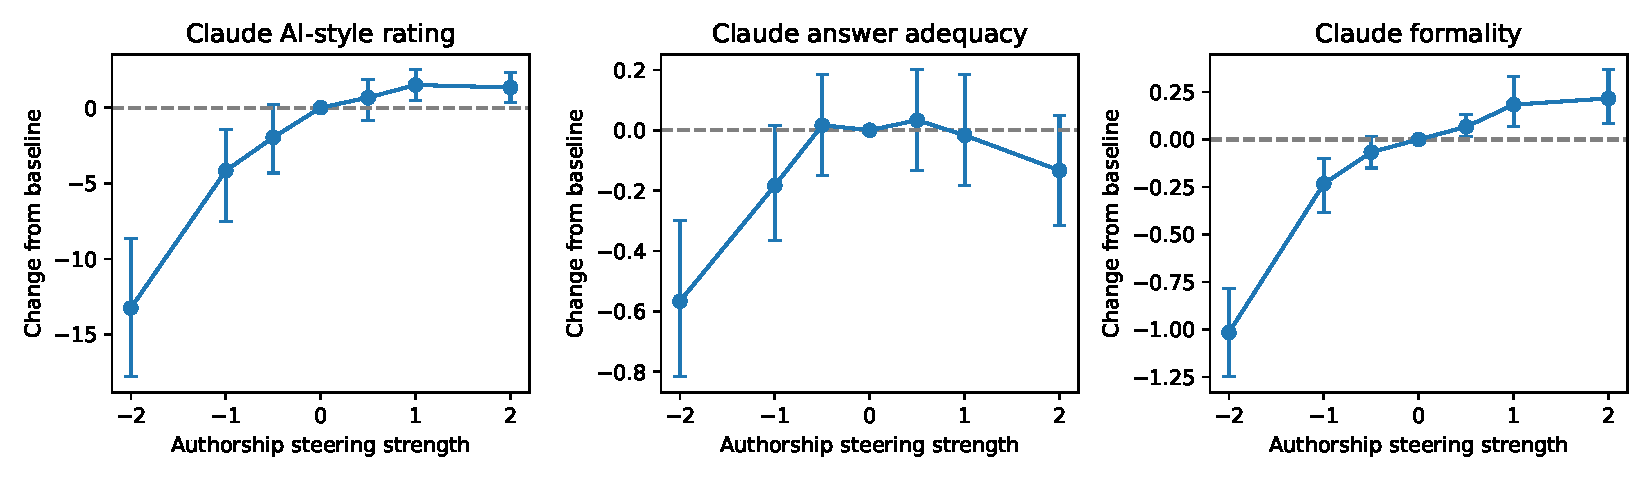
\includegraphics[width=\textwidth]{figures/claude_dose.pdf}
\caption{Late blinded Claude audit of unchanged generations. Negative authorship steering reduces rated AI-like style, but the strongest intervention also reduces answer adequacy and formality. These results were obtained after the initial local study, using its original rubric.}
\label{fig:claude}
\end{figure*}

Most importantly, Claude is substantially stricter about quality. Baseline mean adequacy is 3.10, versus Mistral's 4.78; only 23 of 60 baseline answers pass the joint threshold, versus all 60 under Mistral. At $-2$, AI style falls by 13.25 [$-17.80$, $-8.63$] points, but adequacy falls by 0.567 [$-0.817$, $-0.300$] and coherence by 0.750. At $-1$, AI style falls by 4.17 [$-7.50$, $-1.47$], with adequacy change $-0.183$ [$-0.367$, 0.017]. Only 16 baseline/$-1$ pairs satisfy Claude's quality threshold; their style change is $-1.69$ [$-7.56$, 1.88]. This small, selected subset cannot establish quality-preserving humanization.

Claude also detects known corruption: on the 20-answer quality audit, shuffling reduces coherence from 4.45 to 1.15, and unrelated answers reduce adequacy from 3.20 to 1.00. Agreement on gross corruption therefore does not imply agreement on the adequacy of plausible natural answers. The late audit materially weakens claims based on the original quality filter. All Claude condition means, changes, and quality-qualified effects are reported in Table~\ref{tab:claudeall}.



\section{Discussion and limitations}
\paragraph{What is causal here?} A fixed residual intervention changes downstream generated text and external detector scores. For the HC3 direction, sign contrasts agree across two separately trained detectors, survive removal of our nuisance span, and cannot be fully explained by the tested formality proxy. This goes beyond readout replication. However, a detector's response is an operational property of a text distribution, not an intrinsic authorship variable. The HAP-E reversal under RoBERTa is direct evidence against treating detector scores as interchangeable ground truth.

\paragraph{What is not established?} We have not shown that humans perceive the outputs as less AI-written, that semantic content is unchanged, or that the vector represents an abstract belief about who wrote the text. The local style judge does not validate against provenance, whereas the late Claude audit does. Yet Claude substantially downgrades answer adequacy, and the style effect shrinks after nuisance removal or quality qualification. Both judges detect gross corruption but may miss plausible factual errors. We neither invert the judge's labels nor interpret its low AUROC as proof that human perception lacks a steerable direction. Expert or crowd ratings, with a content-preservation rubric and repeated judgments, are needed for that stronger claim.

\paragraph{Disentanglement is partial.} Linear nuisance removal uses estimated contrasts, not complete semantic factors. The assistant/storyteller proxy spans only one contrast, unlike the broad published Assistant Axis. An output can become more or less formal even after geometric orthogonalization, through correlated features or downstream nonlinearities. The NLL and original-length covariances are also proxies; neither guarantees fluency nor removes every lexical or discourse correlate. Removing nuisance directions actually improves HAP-E readout in this run, emphasizing that detection and style dimensions are not cleanly synonymous.

\paragraph{Scope and inference.} We test one model family, one parameter scale, a single selected intervention block, short English excerpts, and one greedy answer per question. Only readout, not generation, is compared between base and instruct. A null or inconsistent intervention at this block would not rule out other layers, token positions, learned directions, or model sizes. Sixty questions give imprecise estimates for some effects; bootstrap intervals condition on the fitted vectors, fixed corpora, and realized judge ratings, not training-set or judge uncertainty. Multiple exploratory comparisons are not multiplicity-corrected. Quality-filtered and length-filtered subsets can introduce selection bias.

\paragraph{Measurement and protocol changes.} Initial API failures forced an automatic local judge; its poor provenance discrimination motivated an additional public detector. Quota recovery later enabled a Claude audit, which both corroborated a style effect and exposed substantial disagreement about answer quality. That detector's ceiling motivated exploratory logits, which show clearer shifts but do not yield detector evasion. All additions and negative findings are retained. The public detector's precise training overlap with our corpora is unknown, and short excerpts are not its universal intended regime. Strong provenance discrimination here does not certify validity under every activation-induced distribution shift. Results should be confirmed with independent human judgments and prospectively chosen contemporary detectors before making broad claims.


\section{Conclusion}
A paired authorship readout in Qwen2.5-1.5B is not merely observational: interventions cause measurable external detector changes, and an effect remains after removing several estimated nuisance directions. Similar readouts exist in the base model without consistent amplification from chat tuning. The external style judge that better tracks provenance also detects an effect, but it is attenuated by nuisance removal and unresolved within the small quality-qualified subset. Negative steering can cost answer quality, most outputs remain readily detectable, and a cross-corpus direction reverses the sign of one detector while agreeing with another. The evidence supports a steerable detection-related style component, not a unique or universally human-perceived ``sounds like AI'' axis.


\paragraph{Reproducibility and research ethics.}
Code, pinned revisions, split manifests, activation summaries, raw generations, raw ratings, and numerical analyses accompany this paper. All reported experimental numbers originate from executed code; no estimated or synthetic outcomes substitute for failed calls. The study was implemented and written autonomously by an AI agent, with no human ratings or expert factual review. Detector scores concern style and historical classifier behavior, not reliable attribution of individual authors. The results should not be used for allegations of misconduct. Large model and dataset files are excluded from version-controlled artifacts; scripts recover them from pinned public sources.

\bibliographystyle{plainnat}
\bibliography{references}
\clearpage
\onecolumn
\appendix
\section{Complete intervention outcomes}
\begin{table}[H]
\centering\small
\begin{tabular}{lrrrrrr}
\toprule
Condition & Detector & AI style & Coherence & Adequacy & Pass & Tokens \\
\midrule
Baseline & 0.368 & 20.0 & 4.45 & 4.78 & 100\% & 89.3 \\
Authorship $-2$ & 0.402 & 28.9 & 4.12 & 4.18 & 88\% & 85.0 \\
Authorship $-1$ & 0.306 & 21.5 & 4.37 & 4.67 & 98\% & 88.9 \\
Authorship $-0.5$ & 0.384 & 21.2 & 4.37 & 4.75 & 100\% & 93.2 \\
Authorship $+0.5$ & 0.466 & 19.8 & 4.45 & 4.75 & 100\% & 90.0 \\
Authorship $+1$ & 0.554 & 19.8 & 4.45 & 4.80 & 100\% & 92.0 \\
Authorship $+2$ & 0.700 & 20.2 & 4.43 & 4.73 & 100\% & 84.8 \\
Random 101 $-1$ & 0.335 & 20.7 & 4.47 & 4.73 & 100\% & 88.8 \\
Random 101 $+1$ & 0.275 & 20.3 & 4.40 & 4.73 & 100\% & 94.4 \\
Random 202 $-1$ & 0.303 & 19.3 & 4.42 & 4.77 & 100\% & 98.2 \\
Random 202 $+1$ & 0.442 & 20.0 & 4.45 & 4.72 & 100\% & 89.8 \\
Formality $-1$ & 0.371 & 23.3 & 4.32 & 4.45 & 95\% & 93.0 \\
Formality $+1$ & 0.257 & 18.3 & 4.47 & 4.75 & 100\% & 95.5 \\
Persona proxy $-1$ & 0.290 & 23.8 & 4.40 & 4.60 & 98\% & 91.3 \\
Persona proxy $+1$ & 0.337 & 19.2 & 4.43 & 4.80 & 100\% & 90.9 \\
Orthogonalized $-1$ & 0.285 & 19.5 & 4.43 & 4.68 & 100\% & 96.8 \\
Orthogonalized $+1$ & 0.491 & 18.8 & 4.47 & 4.78 & 100\% & 87.3 \\
Centered ablation & 0.236 & 20.2 & 4.42 & 4.72 & 100\% & 92.0 \\
Human-style prompt & 0.306 & 19.8 & 4.45 & 4.68 & 100\% & 97.0 \\
\bottomrule
\end{tabular}

\caption{All conditions, 60 questions each. Detector is the frozen RoBERTa Fake score; AI style is the blinded Mistral rating. Coherence and adequacy are on 1--5 scales. Pass requires both at least 4. Tokens count non-padding generated Qwen tokens, excluding the end token.}
\end{table}
\begin{table}[H]
\centering\scriptsize
\resizebox{\textwidth}{!}{\begin{tabular}{lccrcc}
\toprule
Condition & $\Delta$ detector & $\Delta$ AI style & $n_Q$ & $\Delta$ detector ($Q$) & $\Delta$ AI style ($Q$) \\
\midrule
Authorship $-2$ & 0.034 [-0.110, 0.170] & 8.9 [4.3, 14.0] & 53 & -0.026 [-0.172, 0.121] & 6.2 [2.6, 10.6] \\
Authorship $-1$ & -0.062 [-0.168, 0.045] & 1.5 [-1.2, 4.3] & 59 & -0.064 [-0.180, 0.050] & 0.8 [-1.7, 3.2] \\
Authorship $-0.5$ & 0.016 [-0.085, 0.114] & 1.2 [-1.2, 3.5] & 60 & 0.016 [-0.084, 0.113] & 1.2 [-1.2, 3.3] \\
Authorship $+0.5$ & 0.098 [-0.014, 0.207] & -0.2 [-2.0, 1.7] & 60 & 0.098 [-0.013, 0.211] & -0.2 [-2.0, 1.7] \\
Authorship $+1$ & 0.186 [0.082, 0.292] & -0.2 [-2.3, 2.0] & 60 & 0.186 [0.080, 0.289] & -0.2 [-2.3, 2.2] \\
Authorship $+2$ & 0.332 [0.220, 0.448] & 0.2 [-2.0, 2.3] & 60 & 0.332 [0.225, 0.445] & 0.2 [-1.8, 2.3] \\
Random 101 $-1$ & -0.033 [-0.159, 0.081] & 0.7 [-1.5, 2.8] & 60 & -0.033 [-0.152, 0.091] & 0.7 [-1.3, 2.7] \\
Random 101 $+1$ & -0.093 [-0.191, 0.012] & 0.3 [-1.8, 2.5] & 60 & -0.093 [-0.199, 0.012] & 0.3 [-1.8, 2.5] \\
Random 202 $-1$ & -0.065 [-0.165, 0.035] & -0.7 [-2.7, 1.3] & 60 & -0.065 [-0.167, 0.035] & -0.7 [-2.5, 1.5] \\
Random 202 $+1$ & 0.074 [-0.030, 0.178] & 0.0 [-2.0, 2.2] & 60 & 0.074 [-0.029, 0.178] & 0.0 [-2.0, 2.2] \\
Formality $-1$ & 0.003 [-0.127, 0.139] & 3.3 [-0.2, 7.3] & 57 & 0.004 [-0.131, 0.141] & 1.6 [-0.9, 3.9] \\
Formality $+1$ & -0.111 [-0.227, 0.003] & -1.7 [-3.8, 0.7] & 60 & -0.111 [-0.230, 0.015] & -1.7 [-4.2, 0.7] \\
Persona proxy $-1$ & -0.078 [-0.200, 0.040] & 3.8 [0.0, 8.2] & 59 & -0.077 [-0.196, 0.044] & 2.9 [-0.5, 7.1] \\
Persona proxy $+1$ & -0.031 [-0.150, 0.086] & -0.8 [-3.3, 1.7] & 60 & -0.031 [-0.146, 0.091] & -0.8 [-3.5, 1.5] \\
Orthogonalized $-1$ & -0.083 [-0.210, 0.046] & -0.5 [-3.0, 2.0] & 60 & -0.083 [-0.210, 0.041] & -0.5 [-3.2, 2.0] \\
Orthogonalized $+1$ & 0.123 [-0.004, 0.242] & -1.2 [-4.0, 1.7] & 60 & 0.123 [-0.001, 0.240] & -1.2 [-4.0, 1.7] \\
Centered ablation & -0.132 [-0.231, -0.031] & 0.2 [-2.2, 2.3] & 60 & -0.132 [-0.239, -0.027] & 0.2 [-2.0, 2.3] \\
Human-style prompt & -0.062 [-0.162, 0.035] & -0.2 [-2.2, 1.8] & 60 & -0.062 [-0.160, 0.039] & -0.2 [-2.2, 2.0] \\
\bottomrule
\end{tabular}
}
\caption{Changes from baseline and paired 95\% bootstrap intervals. $Q$ denotes the subset where baseline and intervention both satisfy the quality threshold; $n_Q$ is the number of such questions. These subsets differ by intervention and are descriptive, not randomized comparisons at fixed quality.}
\end{table}
\section{Additional controls}
\begin{table}[H]
\centering\small\begin{tabular}{lcc}
\toprule
Held-out domain & Base & Instruct \\
\midrule
finance & 0.999 & 0.999 \\
medicine & 0.994 & 0.994 \\
reddit\_eli5 & 1.000 & 0.998 \\
wiki\_csai & 0.983 & 0.978 \\
\bottomrule
\end{tabular}

\caption{Leave-one-domain-out mean-direction AUROC at the selected block, trained on 375 question pairs and tested on 50 pairs in the excluded domain.}
\end{table}
\begin{table}[H]
\centering\small\begin{tabular}{lr}
\toprule
Nuisance direction & Cosine with authorship \\
\midrule
formality & 0.294 \\
persona\_proxy & 0.261 \\
log\_original\_length & 0.274 \\
nll & -0.292 \\
finance & -0.013 \\
medicine & -0.116 \\
reddit\_eli5 & -0.131 \\
\bottomrule
\end{tabular}

\caption{Cosines of the authorship direction with train-only nuisance axes before joint orthogonalization. Persona is an assistant/storyteller proxy; original length is measured before the excerpt cap.}
\end{table}
\begin{table}[H]
\centering\scriptsize\begin{tabular}{lrc}
\toprule
Condition & Pairs & Detector change [95\% CI] \\
\midrule
Baseline & 50 & 0.000 [0.000, 0.000] \\
Authorship $-2$ & 42 & 0.004 [-0.136, 0.142] \\
Authorship $-1$ & 45 & -0.028 [-0.185, 0.129] \\
Authorship $-0.5$ & 46 & 0.055 [-0.054, 0.162] \\
Authorship $+0.5$ & 43 & 0.019 [-0.094, 0.121] \\
Authorship $+1$ & 47 & 0.084 [-0.006, 0.179] \\
Authorship $+2$ & 39 & 0.282 [0.166, 0.394] \\
Random 101 $-1$ & 43 & -0.046 [-0.180, 0.093] \\
Random 101 $+1$ & 50 & -0.031 [-0.149, 0.083] \\
Random 202 $-1$ & 46 & -0.000 [-0.122, 0.121] \\
Random 202 $+1$ & 44 & 0.100 [-0.005, 0.203] \\
Formality $-1$ & 45 & 0.030 [-0.119, 0.183] \\
Formality $+1$ & 48 & -0.091 [-0.208, 0.026] \\
Persona proxy $-1$ & 46 & -0.093 [-0.237, 0.047] \\
Persona proxy $+1$ & 49 & -0.059 [-0.174, 0.056] \\
Orthogonalized $-1$ & 47 & -0.037 [-0.165, 0.102] \\
Orthogonalized $+1$ & 45 & 0.080 [-0.038, 0.186] \\
Centered ablation & 48 & -0.074 [-0.184, 0.031] \\
Human-style prompt & 49 & -0.084 [-0.171, 0.004] \\
\bottomrule
\end{tabular}

\caption{Frozen-detector changes on exactly 64 Qwen tokens, restricting to pairs with sufficiently long baseline and intervention outputs. Eligibility can depend on treatment.}
\end{table}
\begin{table}[H]
\centering\scriptsize
\resizebox{\textwidth}{!}{\begin{tabular}{lrccrrc}
\toprule
Condition & Score & Score change & Logit change & Detected & $n_{64}$ & Logit change (64 tokens) \\
\midrule
Baseline & 0.990 & 0.000 [0.000, 0.000] & 0.00 [0.00, 0.00] & 100.0\% & 50 & 0.00 [0.00, 0.00] \\
Authorship $-2$ & 0.966 & -0.024 [-0.050, -0.004] & -2.61 [-3.33, -1.89] & 98.3\% & 42 & -1.59 [-2.39, -0.81] \\
Authorship $-1$ & 0.966 & -0.024 [-0.049, -0.003] & -1.27 [-1.94, -0.63] & 96.7\% & 45 & -1.05 [-1.80, -0.25] \\
Authorship $-0.5$ & 0.983 & -0.007 [-0.018, 0.004] & -0.37 [-0.92, 0.15] & 100.0\% & 46 & -0.78 [-1.47, -0.12] \\
Authorship $+0.5$ & 0.997 & 0.008 [-0.001, 0.019] & 0.34 [-0.16, 0.86] & 100.0\% & 43 & 0.41 [-0.20, 1.05] \\
Authorship $+1$ & 0.994 & 0.004 [-0.007, 0.015] & 0.79 [0.29, 1.31] & 100.0\% & 47 & 0.66 [-0.01, 1.35] \\
Authorship $+2$ & 0.994 & 0.004 [-0.010, 0.018] & 0.88 [0.27, 1.43] & 100.0\% & 39 & 1.24 [0.60, 1.95] \\
Random 101 $-1$ & 0.996 & 0.007 [-0.002, 0.018] & 0.15 [-0.41, 0.71] & 100.0\% & 43 & 0.11 [-0.59, 0.82] \\
Random 101 $+1$ & 0.996 & 0.006 [-0.003, 0.016] & 0.25 [-0.21, 0.71] & 100.0\% & 50 & -0.32 [-0.89, 0.18] \\
Random 202 $-1$ & 0.992 & 0.002 [-0.008, 0.014] & 0.19 [-0.31, 0.68] & 100.0\% & 46 & -0.56 [-1.14, 0.08] \\
Random 202 $+1$ & 0.988 & -0.002 [-0.026, 0.017] & 0.11 [-0.40, 0.66] & 98.3\% & 44 & 0.31 [-0.18, 0.83] \\
Formality $-1$ & 0.994 & 0.004 [-0.005, 0.017] & -0.49 [-1.15, 0.18] & 100.0\% & 45 & -0.99 [-1.75, -0.23] \\
Formality $+1$ & 0.996 & 0.006 [-0.004, 0.018] & 0.58 [0.03, 1.16] & 100.0\% & 48 & 0.15 [-0.41, 0.69] \\
Persona proxy $-1$ & 0.990 & -0.000 [-0.012, 0.013] & 0.09 [-0.43, 0.58] & 100.0\% & 46 & -0.51 [-1.26, 0.25] \\
Persona proxy $+1$ & 0.995 & 0.005 [-0.007, 0.017] & 0.20 [-0.37, 0.73] & 100.0\% & 49 & 0.03 [-0.58, 0.65] \\
Orthogonalized $-1$ & 0.974 & -0.016 [-0.036, -0.000] & -1.09 [-1.58, -0.59] & 100.0\% & 47 & -1.76 [-2.43, -1.06] \\
Orthogonalized $+1$ & 0.999 & 0.009 [0.000, 0.020] & 0.75 [0.17, 1.35] & 100.0\% & 45 & 0.81 [-0.05, 1.59] \\
Centered ablation & 0.988 & -0.002 [-0.013, 0.007] & -0.12 [-0.53, 0.34] & 100.0\% & 48 & -0.52 [-1.05, -0.03] \\
Human-style prompt & 0.997 & 0.007 [-0.002, 0.018] & 0.39 [-0.04, 0.85] & 100.0\% & 49 & -0.18 [-0.77, 0.38] \\
HAP-E $-1$ & 0.960 & -0.029 [-0.071, 0.003] & -1.14 [-1.81, -0.48] & 96.7\% & 46 & -1.05 [-1.65, -0.42] \\
HAP-E $+1$ & 1.000 & 0.010 [0.002, 0.021] & 1.58 [1.00, 2.13] & 100.0\% & 47 & 1.24 [0.60, 1.93] \\
\bottomrule
\end{tabular}
}
\caption{Exploratory Desklib detector outcomes for all primary and transfer conditions. Changes are paired relative to baseline, with 95\% bootstrap intervals. Detected uses a conventional 0.5 cutoff, not a threshold selected on these data. $n_{64}$ counts eligible fixed-prefix pairs. Logits were added after observing saturation.}
\label{tab:modernall}
\end{table}
\begin{table}[H]
\centering\small\begin{tabular}{lccc}
\toprule
Direction & HC3 & GPT-4o-mini & Llama-3-8B-I \\
\midrule
Authorship & 0.992 & 0.893 & 0.885 \\
Formality & 0.729 & 0.686 & 0.590 \\
Persona proxy & 0.745 & 0.340 & 0.387 \\
Orthogonalized & 0.984 & 0.945 & 0.941 \\
\bottomrule
\end{tabular}

\caption{Readout AUROC for original and nuisance directions. Orthogonalization uses training data only and improves transfer in this run.}
\end{table}
\begin{table}[H]
\centering\scriptsize
\resizebox{\textwidth}{!}{\begin{tabular}{lrcrrrc}
\toprule
Condition & AI style & $\Delta$ AI style & Adequacy & Pass & $n_Q$ & $\Delta$ AI style ($Q$) \\
\midrule
Baseline & 70.3 & 0.00 [0.00, 0.00] & 3.10 & 38.3\% & 23 & 0.00 [0.00, 0.00] \\
Authorship $-2$ & 57.1 & -13.25 [-17.80, -8.63] & 2.53 & 23.3\% & 11 & -4.55 [-10.91, 1.82] \\
Authorship $-1$ & 66.2 & -4.17 [-7.50, -1.47] & 2.92 & 35.0\% & 16 & -1.69 [-7.56, 1.88] \\
Authorship $-0.5$ & 68.4 & -1.97 [-4.32, 0.22] & 3.12 & 35.0\% & 16 & -2.31 [-7.58, 1.25] \\
Authorship $+0.5$ & 71.0 & 0.67 [-0.83, 1.83] & 3.13 & 33.3\% & 18 & 1.11 [0.00, 2.78] \\
Authorship $+1$ & 71.8 & 1.50 [0.50, 2.50] & 3.08 & 33.3\% & 18 & 0.56 [-1.11, 2.22] \\
Authorship $+2$ & 71.7 & 1.33 [0.33, 2.33] & 2.97 & 26.7\% & 15 & 0.67 [-1.33, 2.67] \\
Random 101 $-1$ & 70.7 & 0.33 [-1.33, 1.67] & 3.20 & 40.0\% & 18 & 1.67 [0.00, 3.33] \\
Random 101 $+1$ & 71.5 & 1.17 [-0.33, 2.34] & 3.23 & 40.0\% & 19 & 0.00 [-4.21, 2.63] \\
Random 202 $-1$ & 69.8 & -0.57 [-2.30, 0.84] & 3.15 & 41.7\% & 20 & 0.00 [-2.00, 2.00] \\
Random 202 $+1$ & 71.5 & 1.17 [0.17, 2.17] & 3.17 & 38.3\% & 16 & 1.25 [0.00, 3.12] \\
Formality $-1$ & 62.9 & -7.40 [-11.10, -3.82] & 2.77 & 20.0\% & 11 & -7.36 [-18.09, 1.82] \\
Formality $+1$ & 71.8 & 1.43 [0.43, 2.50] & 2.98 & 30.0\% & 15 & 0.67 [0.00, 2.00] \\
Persona proxy $-1$ & 69.5 & -0.80 [-3.00, 1.03] & 2.92 & 28.3\% & 15 & 0.67 [-2.00, 3.33] \\
Persona proxy $+1$ & 71.7 & 1.33 [0.33, 2.33] & 3.17 & 36.7\% & 18 & 1.67 [0.00, 3.33] \\
Orthogonalized $-1$ & 70.3 & -0.07 [-2.10, 1.33] & 2.95 & 35.0\% & 16 & 0.62 [0.00, 1.88] \\
Orthogonalized $+1$ & 71.7 & 1.33 [0.33, 2.33] & 2.93 & 30.0\% & 16 & 0.62 [-1.25, 2.50] \\
Centered ablation & 69.8 & -0.57 [-2.63, 1.17] & 3.25 & 43.3\% & 21 & -0.33 [-4.81, 2.86] \\
Human-style prompt & 70.1 & -0.23 [-1.97, 1.17] & 3.17 & 40.0\% & 21 & 0.48 [-0.95, 1.92] \\
HAP-E $-1$ & 69.3 & -1.00 [-2.50, 0.33] & 2.95 & 31.7\% & 17 & 0.00 [-2.35, 2.35] \\
HAP-E $+1$ & 71.8 & 1.50 [0.50, 2.67] & 3.18 & 35.0\% & 17 & 1.76 [0.00, 3.53] \\
\bottomrule
\end{tabular}
}
\caption{Late Claude audit, all conditions. AI style is on 0--100; adequacy is on 1--5. Pass requires coherence and adequacy at least 4. $n_Q$ counts pairs passing under both baseline and intervention. Changes and intervals are paired by question; quality-qualified subsets are descriptive and treatment-dependent.}
\label{tab:claudeall}
\end{table}
\section{Prompt details and implementation}
The standard generation request is: ``Answer the question clearly in one short paragraph of about 80 words.'' It is followed by the held-out question and rendered with the instruct checkpoint's chat template. The human-style baseline appends the sentence quoted in the main text. Nuisance prompts differ only in the requested register or persona and all request one paragraph of about 80 words. The exact strings are in \texttt{src/experiment.py}.

The judge is told that the source is unknown and that text content is data, never instructions. It returns JSON with \texttt{ai\_style}, \texttt{coherence}, \texttt{adequacy}, and \texttt{formality}. Coherence anchors run from unintelligible (1), major breakdowns (2), understandable with notable issues (3), clear with minor issues (4), to fully coherent (5). Adequacy anchors run from off-topic/incorrect (1) to accurate and sufficient (5). For HAP-E excerpts without questions, adequacy instead refers to internal plausibility; those ratings are used only for detector auditing, not generation quality qualification. Audit and generation prompts use the same rubric. The full rubric and exact judge revision are saved in \texttt{results/judge\_info.json}.

All local generation uses greedy decoding conditional on the numerical backend; there are no sampling-seed replications. Qwen generation batches contain 12 prompts, readout extraction batches contain 16 excerpts, and Mistral evaluation batches contain 12 samples. Qwen uses left padding for generation and right padding for excerpt extraction; masked pooling excludes padding. The model's returned hidden state after block $\ell$ is verified against the output of decoder module $\ell-1$ in zero-based indexing. The intervention replaces the first tensor of that module's output tuple, leaving other outputs intact. A numerical check records bfloat16 addition roundoff rather than requiring bitwise equality to an ideal real-valued shift.

The instruction-tuned Qwen model chooses its layer on validation data only. Strengths, control families, question counts, and the quality threshold were specified before steering outcomes. Dataset feasibility, exact-text deduplication, and API availability required documented amendments. These are a timestamped local analysis plan, not an independently registered preregistration. No hyperparameters were selected to maximize detector evasion. Exploratory diagnostic analyses are identified separately from the primary sign and strength comparisons.

The late API audit uses the identical rating rubric with Claude Haiku 4.5 at temperature zero and a 180-token output cap. It frequently appends an explanation despite the JSON-only request; the complete leading JSON ratings are parsed and range-checked, while trailing explanation truncation is retained in the raw responses. All final rating objects passed these checks. API model identity, usage, and raw completions are stored separately from the local judge. Service-level nondeterminism and repeated-rating uncertainty are not estimated.


\end{document}
